In this section, we will discuss the process of obtaining word-context
data and propose a postprocessing transformation which helps to
address a common shortcoming. Using a context distribution for
describing a word seems to imply that the
contexts - used as atomic events in the distribution - are independent
from each other. In practice, that assumption is far from true. For
the sake of concreteness, let us focus on the type of labeling that will be used for
the experimental results - topic models. Therefore, from here on out, we will
refer to contexts as {\em topics}. It is easy to observe
manually, that even for the best topic model one can find a pair of
topics that are closely related and a pair that is much more
distant. Those interrelations between topics are 
properties that represent useful information about the model that is
possible to infer from the data, and yet
may be completely ignored in distributional representations of words. 
For example, we may find a word $w$ that has topic distribution $P_w$
concentrated on a single topic $t$, but it does 
not peak at all other topics that are very similar to
topic $t$. In this case, topic correlations would not be reflected in
the distribution. This shortcoming was observed in \cite{bache:2013},
also in the context of measuring text diversity. We propose a more
general solution to this problem.

Let $p$ be a row vector (corresponding to some word $w$)  from the
word-topic occurrence matrix $\cM_{|V|\times|T|}$ obtained from an LDA
model. We could think of the topics as representing a basis
$t_1,...,t_T$ in some hypothetical vector space $\cH$. In 
this case, $p$ corresponds to a linear combination of the basis
vectors, $\Sigma p_i t_i$. In other words, for every occurrence of
word $w$ labeled with $i$-th topic, we add basis vector $t_i$ to the
complete representation of $w$ in space $\cH$.
Suppose that $\cH$ is a Hiblert space (i.e. has a scalar
product). Now, the correlation between two topics can be represented
by the dot product of the corresponding basis vectors (we assume those
are unit vectors). We can consider a following alternative representation
of a point in $\cH$:

\bed
Let $p\in\rr^T$ be a vector. Denote $x=\sum_{i=1}^T p_i
t_i\in\cH$. Let $\widehat{p}\in\rr^T$ be defined so that
\[\widehat{p}_i = \langle x,t_i\rangle.\]
We will call $\widehat{p}$ the dot-product representation of $p$.
\eed

Notice, that if the considered topic basis is orthonormal, then both
representations $p$ and $\widehat{p}$ are identical. Consider the Gram matrix
$\Sbb=\{\langle t_i,t_j\rangle\}_{i,j}$ of all possible dot products between
basis vectors. If the basis is orthonormal, this is simply the identity
matrix. Moreover, no matter which basis we choose, matrix $\Sbb$ is the
only information we need to translate $p$ to $\widehat{p}$.

\ber
For any vector $p\in\rr^T$, any Hilbert space $\cH$ and a set of
vectors $t_1,...,t_T\in\cH$, we have 
\[\widehat{p} = p\Sbb,\]
where $\Sbb=\{\langle t_i,t_j\rangle\}_{i,j}$ is the Gram matrix.
\eer

The dot-product representation allows us to incorporate the topic
similarity information into a vector representation. Moreover, we do
not need to directly manipulate the space $\cH$ to obtain it, except
computing pairwise topic correlations $s_{ij}$. Once we compute matrix
$\Sbb$, we can transform our data matrix into this new form using simple
matrix multiplication $\cM'=\cM\cdot \Sbb$. Since the co-occurrence matrix
must have nonnegative coefficients, we will require that the matrix
$\Sbb$ also has to be element-wise nonnegative (which it would not
have to be, in general). The new data matrix $\cM'$ can be interpreted
as follows: for each original word-topic co-occurrence, we also add to
the matrix some {\em fractional} co-occurrences of the same word with
other topics, based on their similarity to the main topic.

To obtain a topic similarity matrix, all we need is to write
the topics as nonnegative vectors in a common space. When the topics
come from an LDA model, there is two standard ways to do that: a
distribution over words, or a distribution over documents. Following
the analysis in \cite{bache:2013}, we used the document distributions,
with cosine similarity as a measure of correlation. However, we use the
topic similarities in a different way, that can not only make this
technique applicable to any task relying on distributional word
representations, but also outperforms the aforementioned one for
measuring diversity.

To illustrate the benefit of introducing topic similarities for
measuring diversity, consider a simple case where we have a pair of words
$S=(w_1,w_2)$, with distributional representations $P_1,P_2$, each having
singleton support on one topic (topic similarities not
applied). Clearly, if those topics match, we 
have no diversity, and if they don't, we get relatively high diversity
(assuming uniform weights of the mixture, it would be $\log 2$). Notice, that without introducing topic similarity this is
independent of which pair of topics we are looking at. It could, for
instance, be ``Mathematics'' and ``Physics'' (closely related), or
``Mathematics'' and ``Literature'' (further apart).  Applying the
topic similarity matrix allows for this distinction to be clear and properly
reflected in the results, because the weight from the main topic has
to be redistributed among similar ones, making the distributions $P_1$
and $P_2$ more comparable.
  
  
  \begin{table*}[t]
\begin{center}
\begin{tabular}{CC}
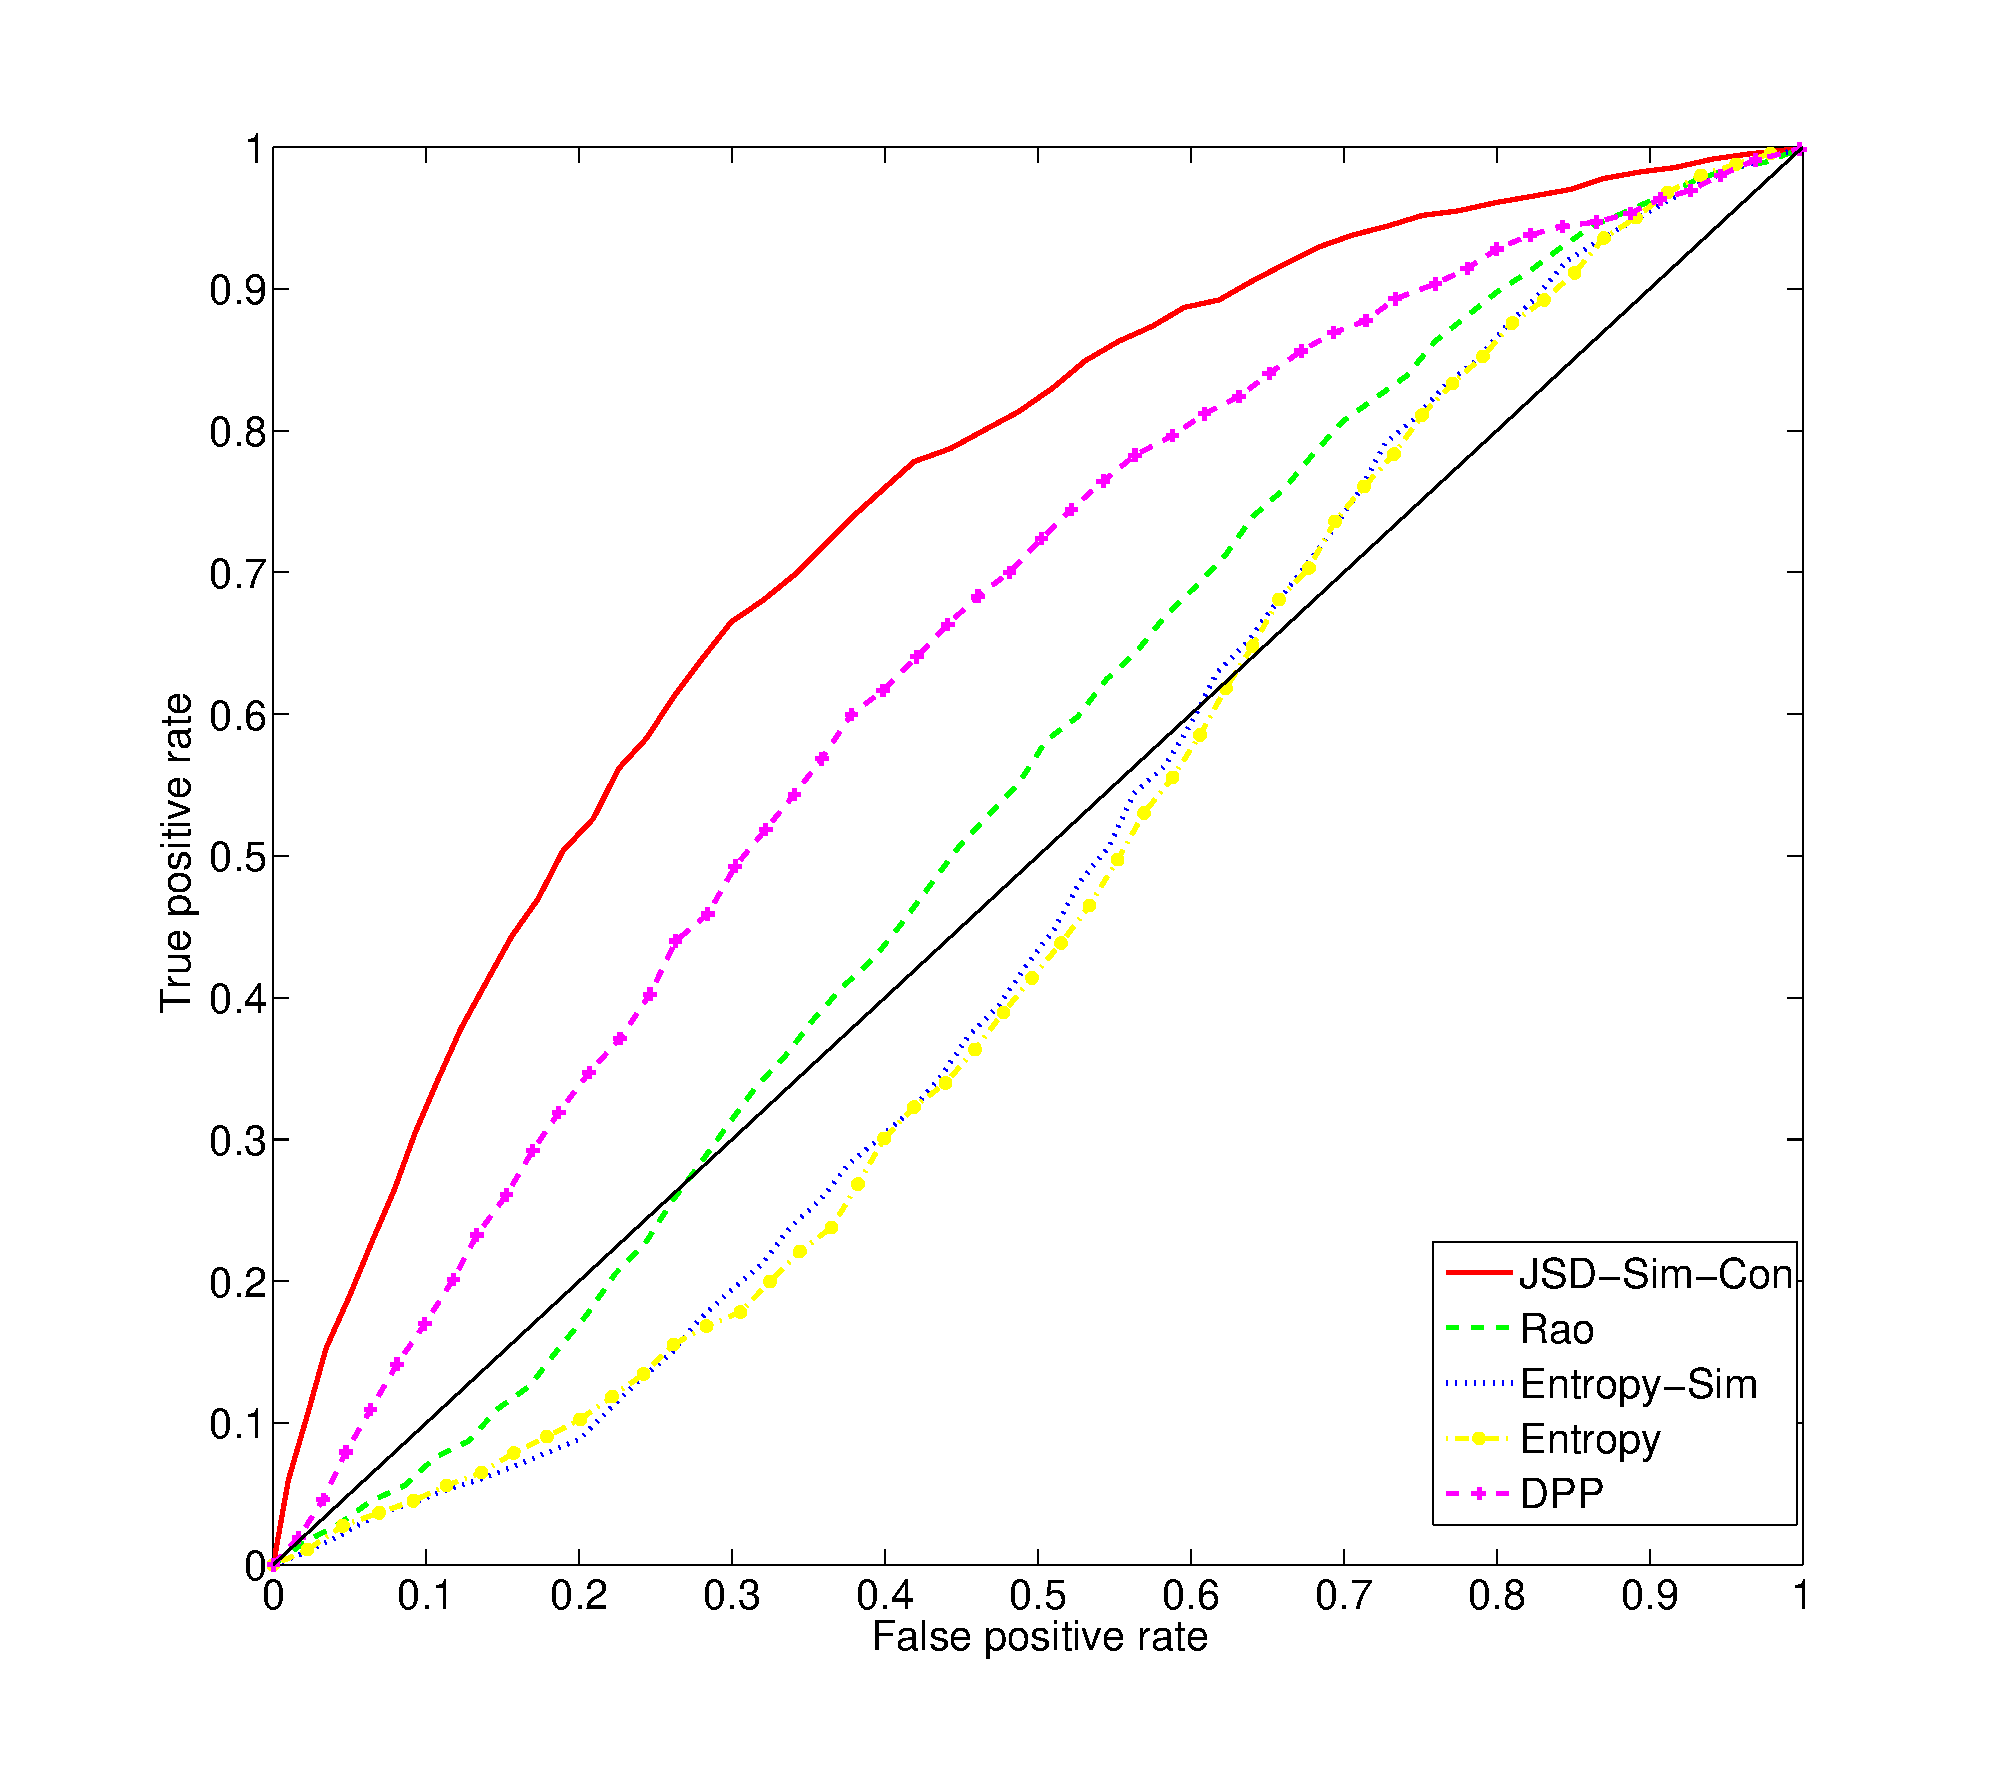
\includegraphics[height=6.5cm]{figures/phonecases-comparison-new.eps}&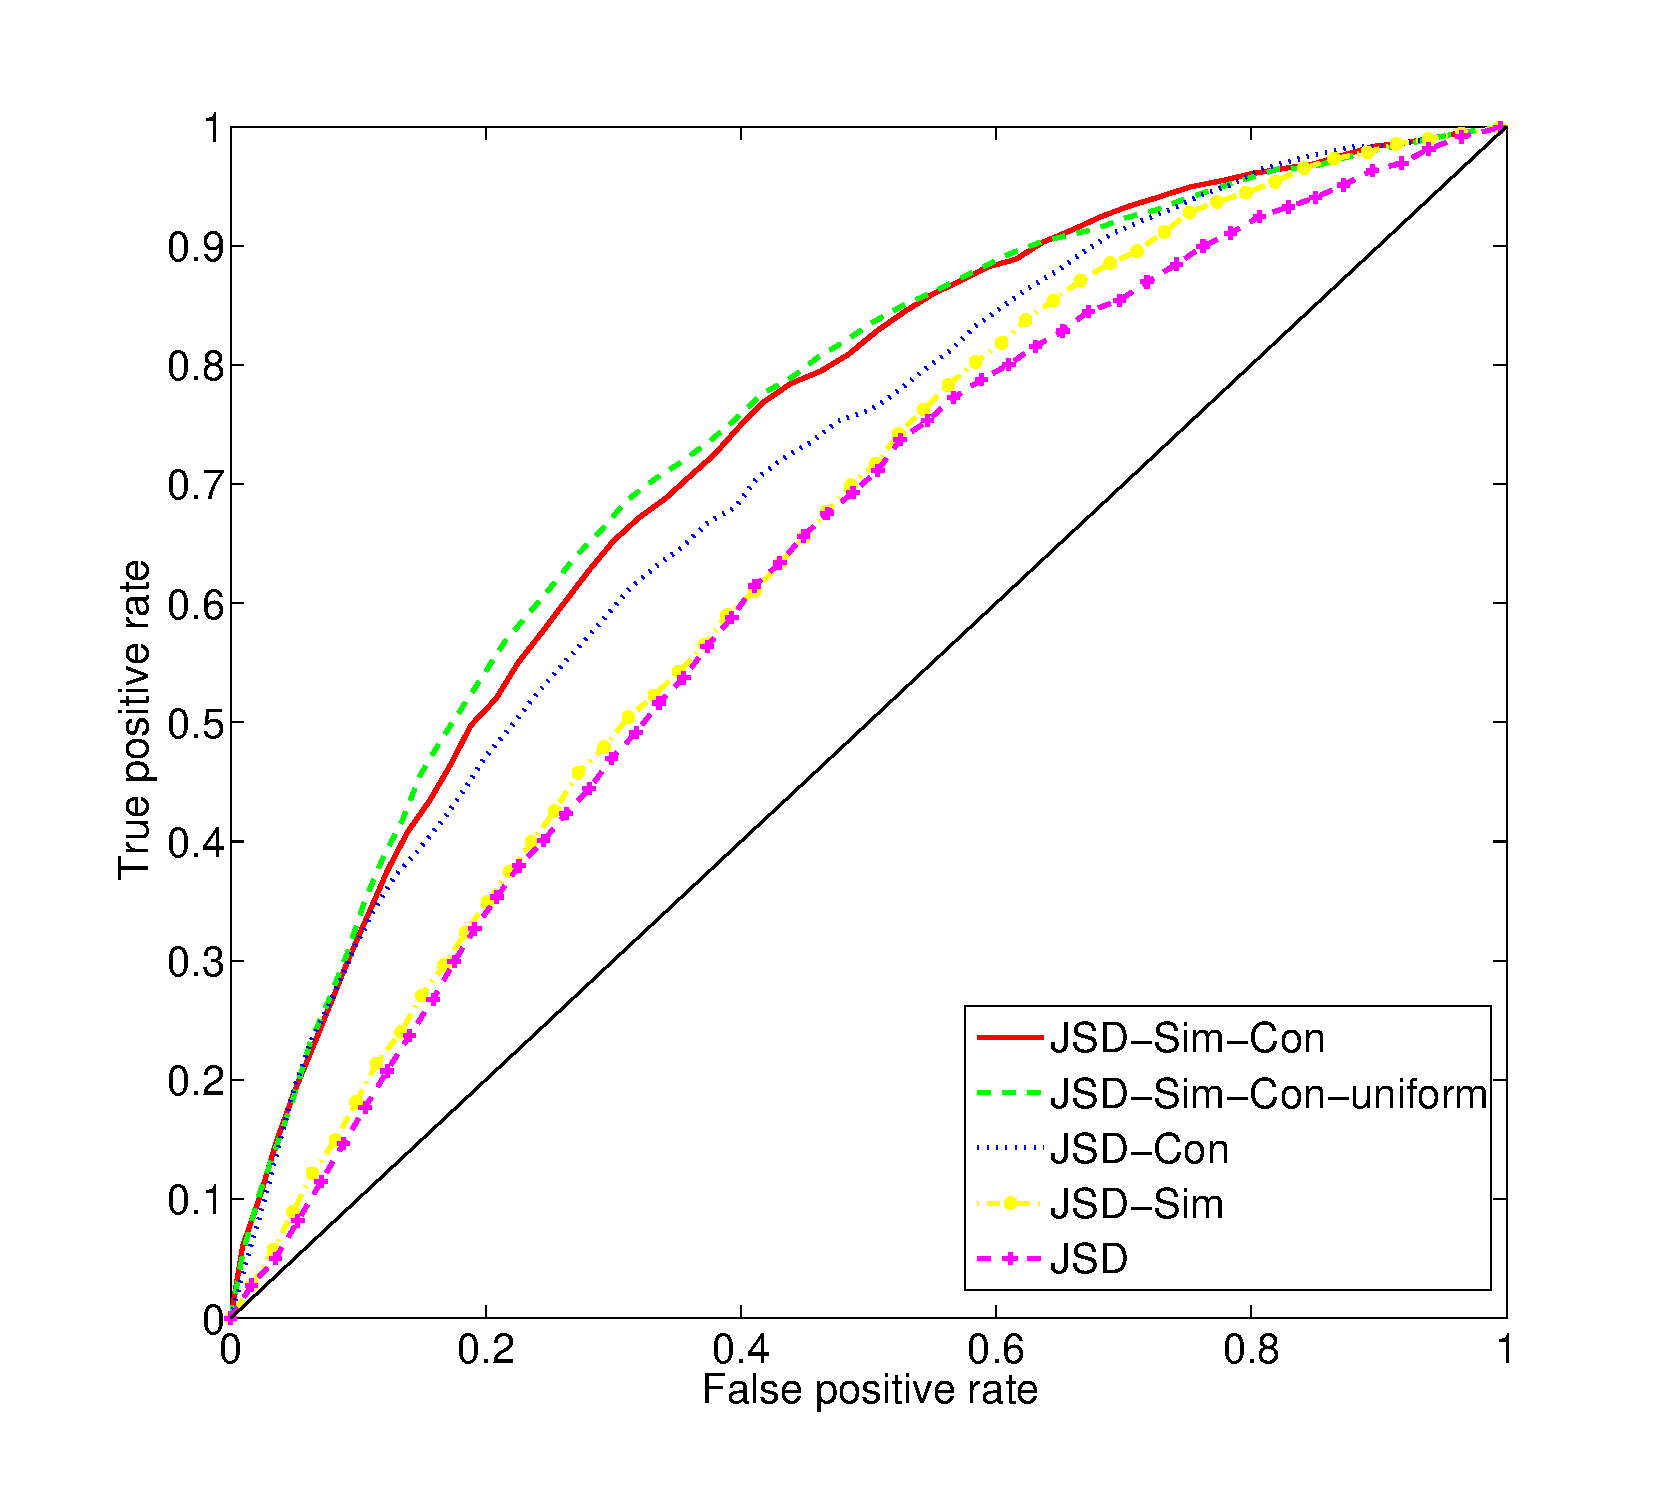
\includegraphics[height=6.5cm]{figures/phonecases-breakdown-new.eps}\\
(a) & (b)\\
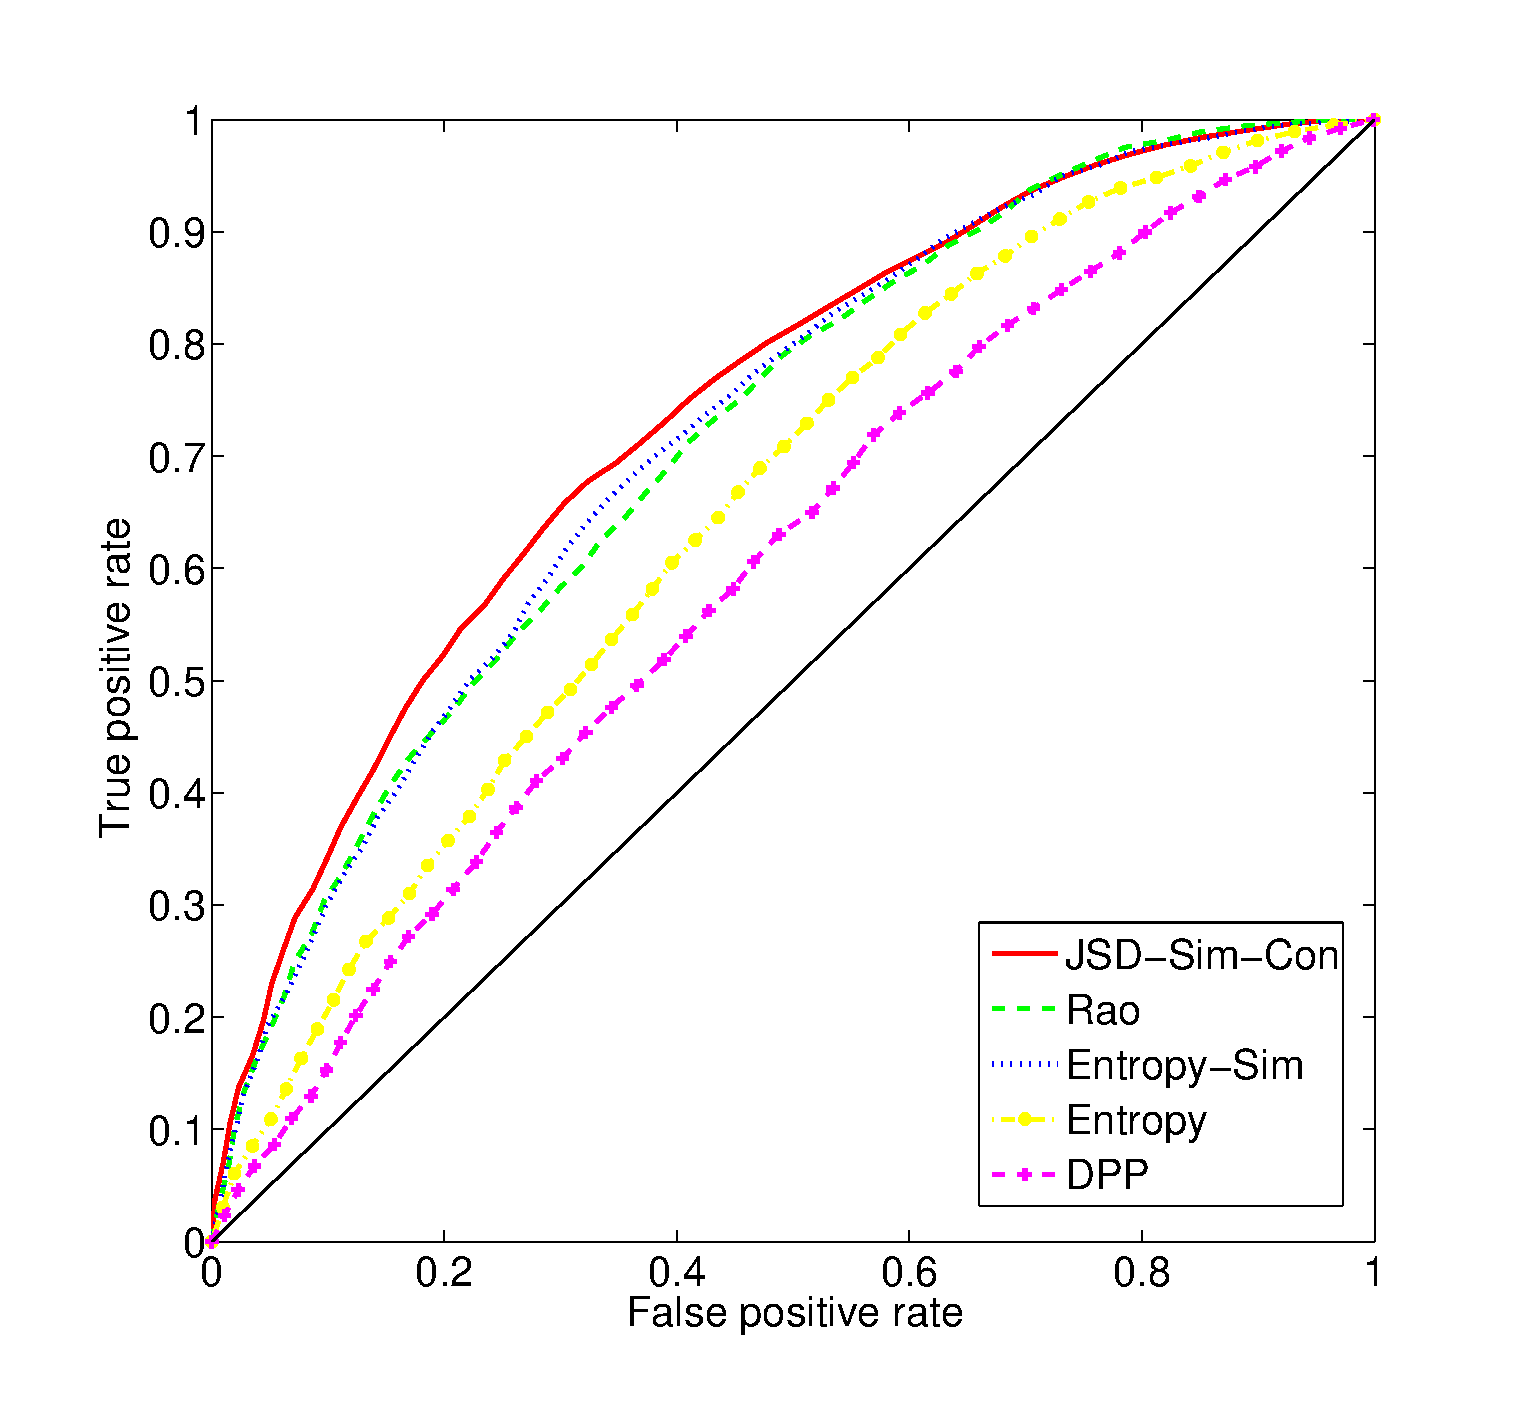
\includegraphics[height=6.5cm]{figures/nsf-comparison-new.eps}&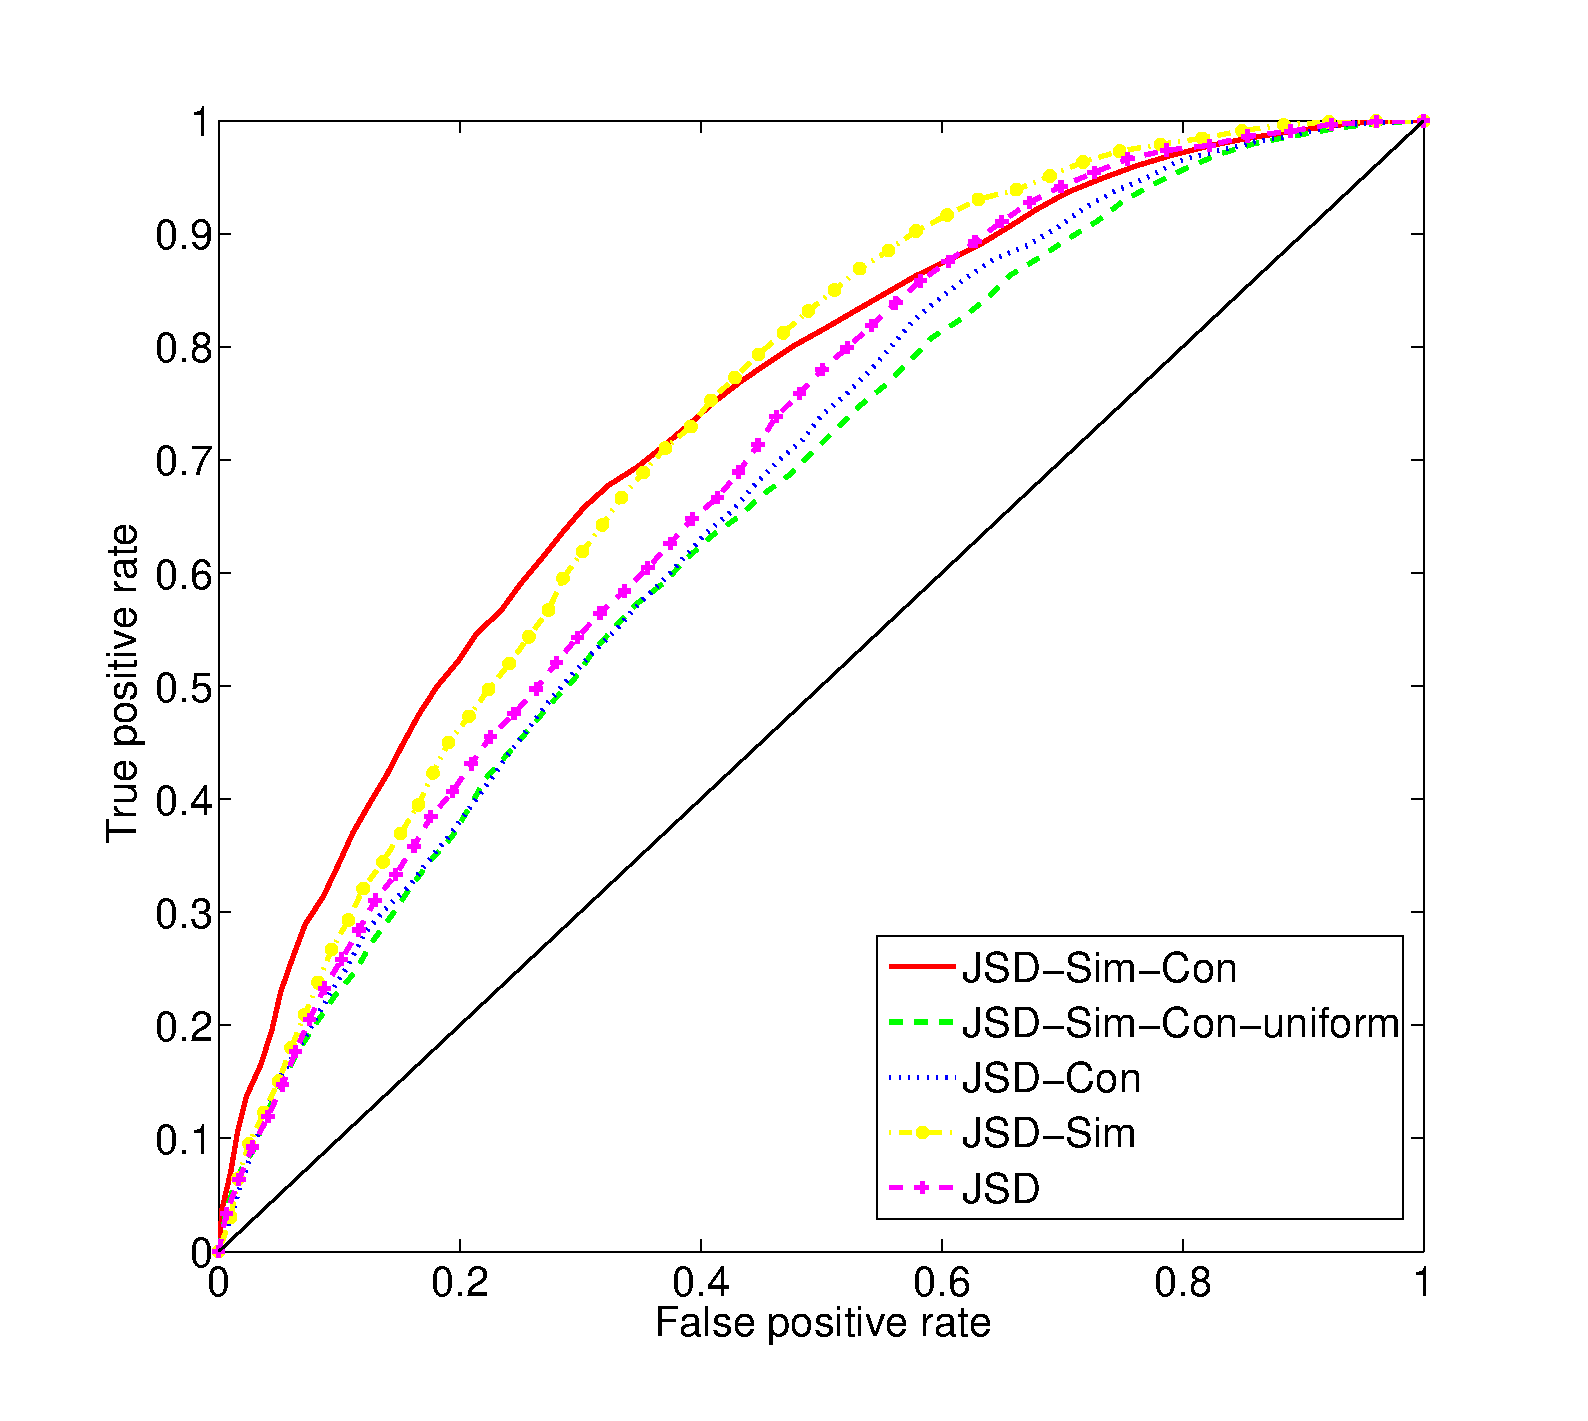
\includegraphics[height=6.5cm]{figures/nsf-breakdown-new.eps}\\
(c) & (d)\\
\end{tabular}
\end{center}
\caption{ROC curves presenting the results of experiments on
the eBay dataset (a,b) and NSF proposal dataset (c,d). The
comparison plots (a,c) show the results for our approach (JSD-Sim-Con)
against other methods, while the plots (b,d)
show different variations of our approach. }
\label{fig:roc-curves}
\end{table*}

